% ============================================================================
% 附录 AF：等离子体湍流与反常输运（注明出处）
% 数值唯一来源：tools/calc/appAF_calc.py -> tools/calc/appAF_calc.txt（本附录所有标出的数字都由它复算）
% 单位写法：量纲用 \mathrm{...}，避免中文字符进数学字体；百分比写成 $0.77663$ 这样的纯数字
% 速度与长度约定：rho_i = sqrt(2 T_i/m_i)/omega_ci（附录 AD/AE 口径）、
%                 rho_s = c_s/omega_ci = rho_i/sqrt(2)（等温电子口径）、
%                 谱用无量纲波数 k_theta rho_s 标注
% 版权口径：只借鉴结论、公式形式与题型；文字、数值、表格自拟并由 tools/calc/appAF_calc.py 独立复算；
%           本书不列 DOI，只给书名/作者/年份/卷期页
% 分工：附录 S 讲约束定标、附录 AE 讲动理学框架、附录 AD 讲台基、附录 AC 讲数值方法；
%       本附录讲「为什么约束就是现在这个数」——湍流机制与反常输运
% ============================================================================

\section{三个输运系数：反常输运到底有多反常}
\label{sec:app-af-scales}

附录 S 给出了约束定标，附录 AE 给出了动理学框架，但两处都跳过了同一个问题：
\textbf{能量到底是怎么从芯部漏出去的}。按碰撞算出来的新经典输运比实验反推的小一到两个数量级，
这个差额就是「反常输运」，而它的来源是湍流。

先把「实验反推」写成可算的量。取 D1 工作点（$n_e=10^{20}$ m$^{-3}$、$T_e=T_i=9.194$ keV、
$B=5.3$ T、$a=2$ m、$\tau_E=3.7$ s），把能量约束时间翻译成扩散系数
\begin{equation}
\chi_{\mathrm{eff}}=\frac{a^2}{2\tau_E}
=0.540541\ \mathrm{m^2\,s^{-1}},
\label{eq:app-af-chieff}
\end{equation}
这就是「装置实测」的那个数。再写三个理论候选：玻姆扩散、用离子回旋半径的回旋玻姆扩散、
和用离子声回旋半径的回旋玻姆扩散
\begin{equation}
\chi_B=\frac{T_e}{16eB}=108.42\ \mathrm{m^2\,s^{-1}},
\qquad
\chi_{gB,i}=\frac{\rho_i^2c_s}{a}=5.07013\ \mathrm{m^2\,s^{-1}},
\label{eq:app-af-chib}
\end{equation}
\begin{equation}
\chi_{gB,s}=\frac{\rho_s^2c_s}{a}=2.53506\ \mathrm{m^2\,s^{-1}},
\label{eq:app-af-chigb}
\end{equation}
三者的比一句话说清：玻姆比实验大 $200.577$ 倍，回旋玻姆（离子口径）大 $9.37973$ 倍
（用离子声口径则是 $4.68987$ 倍）。\textbf{反常输运不等于「随便大」，它被回旋玻姆钉在同一个量级上}——
这正是湍流定标律能用的原因。

\begin{table}[htbp]
\centering
\small
\begin{tabular}{p{3.0cm}p{3.0cm}p{3.2cm}p{4.0cm}}
\toprule
候选 & 本工作点的值 & 对 $B$ 的依赖 & 与实验反推之比 \\
\midrule
玻姆 $\chi_B$ & $108.42$ m$^2$s$^{-1}$ & $1/B$ & $200.577$ \\
回旋玻姆（$\rho_i$） & $5.07013$ m$^2$s$^{-1}$ & $1/B^2$ & $9.37973$ \\
回旋玻姆（$\rho_s$） & $2.53506$ m$^2$s$^{-1}$ & $1/B^2$ & $4.68987$ \\
实验反推 $\chi_{\mathrm{eff}}$ & $0.540541$ m$^2$s$^{-1}$ & —— & $1$ \\
\bottomrule
\end{tabular}
\caption{三个输运系数与实验反推的对比。注意回旋玻姆的两个口径只差一个 $\sqrt{2}$：
$\rho_s=\rho_i/\sqrt{2}$，所以比值差 $2$ 倍。}
\label{tab:app-af-scales}
\end{table}

把这个扩散系数代回功率账，看它是不是「够用」。取梯度长度 $L_T=0.5$ m、迎风面积 $S=489.532$ m$^2$，
\begin{equation}
Q_{\mathrm{turb}}=\frac{n_eT_e\chi_{\mathrm{eff}}}{L_T}
=0.159248\ \mathrm{MW\,m^{-2}},
\qquad
P_{\mathrm{turb}}=Q_{\mathrm{turb}}S=77.9568\ \mathrm{MW},
\label{eq:app-af-q}
\end{equation}
而稳态下的总损失功率是 $W_{\mathrm{th}}/\tau_E=100.378$ MW。也就是说这套粗糙的估算
一次就「解释」了 $0.77663$ 的总损失（相当于 $0.700421$ 的 $\alpha$ 加热功率）——
量级对得上，剩下的差额留给新经典输运、辐射损失和边界。

\begin{tip}{反常输运不是「多了一点」，是两个数量级}{tip-app-af-orders}
$\chi_B/\chi_{\mathrm{eff}}=200.577$ 听起来像「玻姆定标很差」，但真正该记住的是另一半：
回旋玻姆与实验只差 $9.37973$ 倍，而回旋玻姆本身是\textbf{唯一随 $B^2$ 变小的候选}。
磁场翻倍时回旋玻姆降到 $0.25$ 倍、玻姆只降到 $0.5$ 倍——这就是「为什么还要把 $B$ 往上推」。
\end{tip}

{\footnotesize
\textbf{出处：}本节的输运系数分类与回旋玻姆定标参照 Horton \emph{Rev. Mod. Phys.} \textbf{71} (1999) 735 与
Connor \& Wilson \emph{Plasma Phys. Control. Fusion} \textbf{36} (1994) 719。
功率账口径与附录 S、附录 U 一致。
}

\section{漂移波：梯度和磁场谁说了算}
\label{sec:app-af-driftwave}

密度和温度的梯度本身就能让等离子体振荡起来：电子沿磁场方向的自由运动把电荷分离短路掉，
剩下的\textbf{垂直于磁场}的漂移则由梯度方向与磁场方向共同决定。把这件事写成频率，
用离子声回旋半径 $\rho_s=c_s/\omega_{ci}$ 作长度单位最方便
\begin{equation}
\rho_s=\frac{c_s}{\omega_{ci}}=\frac{593524}{2.03071\times10^{8}}
=2.92274\times10^{-3}\ \mathrm{m}=2.92274\ \mathrm{mm},
\qquad
\frac{\rho_s}{\rho_i}=0.707107,
\label{eq:app-af-rhos}
\end{equation}
注意 $\rho_s=\rho_i/\sqrt{2}$ 只是温度相等时的巧合（附录 AE 的 $\rho_i$ 用的是 $\sqrt{2T_i/m_i}$），
换成 $T_i\ne T_e$ 就不再成立。

漂移波的频率与波数成正比、与密度梯度长度成反比，但\textbf{与磁场大小无关}（只要固定无量纲波数
$k_\theta\rho_s$）：把 $k_\theta=k_\theta\rho_s/\rho_s$ 代进去，$\rho_s$ 里的 $1/B$ 正好被抵消
\begin{equation}
\omega_*=\frac{k_\theta T_e}{eBL_n}=k_\theta\rho_s\frac{c_s}{L_n}
=0.3\times\frac{593524}{1.0}=178057\ \mathrm{rad\,s^{-1}},
\label{eq:app-af-omega-star}
\end{equation}
对应频率 $f_*=\omega_*/(2\pi)=28.3387$ kHz，而 $\omega_*/\omega_{ci}=8.76822\times10^{-4}$——
漂移波比离子回旋慢三个量级，所以离子基本是「跟着走」的，这正是回旋动理学能把回旋相位平均掉的前提。

\begin{table}[htbp]
\centering
\small
\begin{tabular}{p{4.2cm}p{3.4cm}p{5.2cm}}
\toprule
量 & 本工作点的值 & 它由什么决定 \\
\midrule
垂直波数 $k_\theta$（$k_\theta\rho_s=0.3$） & $102.643$ m$^{-1}$ & 谱峰的无量纲位置 $\div\rho_s$ \\
垂直波长 $\lambda_\theta$ & $6.12137$ cm & $2\pi/k_\theta$ \\
抗磁漂移速度 $v_{\mathrm{dia}}$ & $1734.72$ m/s & $\rho_sc_s/L_n$ \\
漂移波频率 $\omega_*$ & $178057$ rad/s（$28.3387$ kHz） & $k_\theta\rho_sc_s/L_n$，与 $B$ 无关 \\
环向涡数 $2\pi R/\lambda_\theta$ & $636.389$ 个 & 装置尺寸 $\div$ 垂直波长 \\
\bottomrule
\end{tabular}
\caption{漂移波的尺度表。$k_\theta\rho_s$ 是无量纲量，本附录一律取谱峰位置 $0.3$；
换成别的值只需按比例换算。}
\label{tab:app-af-driftwave}
\end{table}

\begin{tip}{漂移波不是「波」，是梯度与磁场的必然产物}{tip-app-af-driftwave}
有梯度、有磁场，就一定有抗磁漂移；有抗磁漂移、有平行方向的电子响应，就一定有漂移波。
它不需要外部天线去激发——\textbf{是平衡态自己不稳定的那种「必然」}。所以关掉加热不会让它消失，
只会让它换了驱动来源。
\end{tip}

{\footnotesize
\textbf{出处：}漂移波机制与 $\omega_*$ 的推导参照 Wesson \emph{Tokamaks}（第 4 版，2011，第 12 章）。
Helander \& Sigmar \emph{Collisional Transport in Magnetized Plasmas}（2002，第 4 章）与
Horton \emph{Rev. Mod. Phys.} \textbf{71} (1999) 735。
$\rho_s$ 与 $\rho_i$ 的口径与附录 AE 一致。
}

\section{不稳定性：ITG 与 TEM}
\label{sec:app-af-instability}

漂移波本身在纯流体极限下是稳定的，真正让它长起来的是\textbf{梯度里的第二项}：温度梯度。
把温度梯度长度与密度梯度长度之比写成 $\eta_i$
\begin{equation}
\eta_i=\frac{L_n}{L_T}=\frac{1.0}{0.5}=2,
\qquad
\frac{\eta_i}{\eta_{i,\mathrm{crit}}}=\frac{2}{1.5}=1.33333,
\label{eq:app-af-eta}
\end{equation}
其中阈值 $\eta_{i,\mathrm{crit}}=1.5$ 是文献量级（声明值，随磁剪切、安全因子与碰撞率变化）。
离子温度梯度（ITG）模就长在 $\eta_i$ 超过阈值的地方；它靠离子在坏曲率区的漂移共振吸收自由能。

更常用的写法是把梯度归一到装置尺度
\begin{equation}
\frac{R}{L_T}=\frac{6.2}{0.5}=12.4,
\qquad
\frac{R}{L_n}=\frac{6.2}{1.0}=6.2,
\qquad
\frac{1}{L_T}=2\ \mathrm{m^{-1}},
\label{eq:app-af-rlt}
\end{equation}
对应的临界梯度长度是
\begin{equation}
L_{T,\mathrm{crit}}=\frac{R}{(R/L_T)_{\mathrm{crit}}}=\frac{6.2}{5}=1.24\ \mathrm{m},
\qquad
\frac{L_{T,\mathrm{crit}}}{L_T}=2.48,
\label{eq:app-af-ltcrit}
\end{equation}
也就是说本工作点的温度梯度比临界值陡 $2.48$ 倍（超临界幅度 $1.48$）。这里的 $5$ 是
$(R/L_T)_{\mathrm{crit}}$ 的文献量级——临界值本身不是常数，它随 $\eta_i$、磁剪切和 $\rho_i/a$ 漂移。

第二类驱动是\textbf{捕获电子模}（TEM）。电子被磁镜捕获的比例（附录 AE 的 $f_t=0.69843$）
决定了有多少电子参与「慢」的那一支响应
\begin{equation}
f_{\mathrm{trap}}=0.69843,
\qquad
\frac{n_{\mathrm{trap}}}{n_e}=f_{\mathrm{trap}}=0.69843,
\label{eq:app-af-tem}
\end{equation}
捕获电子沿香蕉轨道来回，其平行速度远小于通行电子，于是它们对漂移波的响应相位不同——
这部分相位差就是 TEM 的自由能来源。TEM 与 ITG 的区别不在「有没有梯度」，而在\textbf{谁提供自由能}：
ITG 用离子温度梯度，TEM 用捕获电子对密度与温度梯度的响应。

\begin{table}[htbp]
\centering
\small
\begin{tabular}{p{3.6cm}p{2.8cm}p{2.6cm}p{4.0cm}}
\toprule
判据 & 本工作点 & 阈值（声明） & 结论 \\
\midrule
$\eta_i=L_n/L_T$ & $2$ & $1.5$ & ITG 不稳定（$1.33333$ 倍） \\
$R/L_T$ & $12.4$ & $5$ & 超临界 $1.48$ \\
$L_T$ 与临界值之比 & $0.5$ m & $1.24$ m & 陡 $2.48$ 倍 \\
捕获电子比例 $f_{\mathrm{trap}}$ & $0.69843$ & —— & TEM 有足够驱动 \\
\bottomrule
\end{tabular}
\caption{ITG 与 TEM 的阈值表。阈值的两列要分开看：左边是从本工作点算出来的，
右边是文献量级（声明值），二者相比才有意义。}
\label{tab:app-af-instability}
\end{table}

\begin{tip}{临界梯度不是开关，是刚性}{tip-app-af-stiffness}
刚过阈值时湍流输运只按很小的幂次增长，超过一两倍之后会突然变得非常陡——
这个现象叫「刚性」（stiffness）。它的实际含义是：\textbf{温度剖面会被自己「钉」在临界梯度附近}，
加多少加热功率都主要是把梯度往上顶一点点，而不是把温度顶上去。
这也解释了为什么托卡马克的芯部剖面总是长得差不多。
\end{tip}

{\footnotesize
\textbf{出处：}ITG 与 TEM 的阈值判据参照 Wesson \emph{Tokamaks}（第 4 版，2011，第 12 章）。
Horton \emph{Rev. Mod. Phys.} \textbf{71} (1999) 735 与 Garbet 等
\emph{Plasma Phys. Control. Fusion} \textbf{46} (2004) B557。
捕获比例与附录 AE 同口径。
}

\begin{figure}[htbp]
\centering
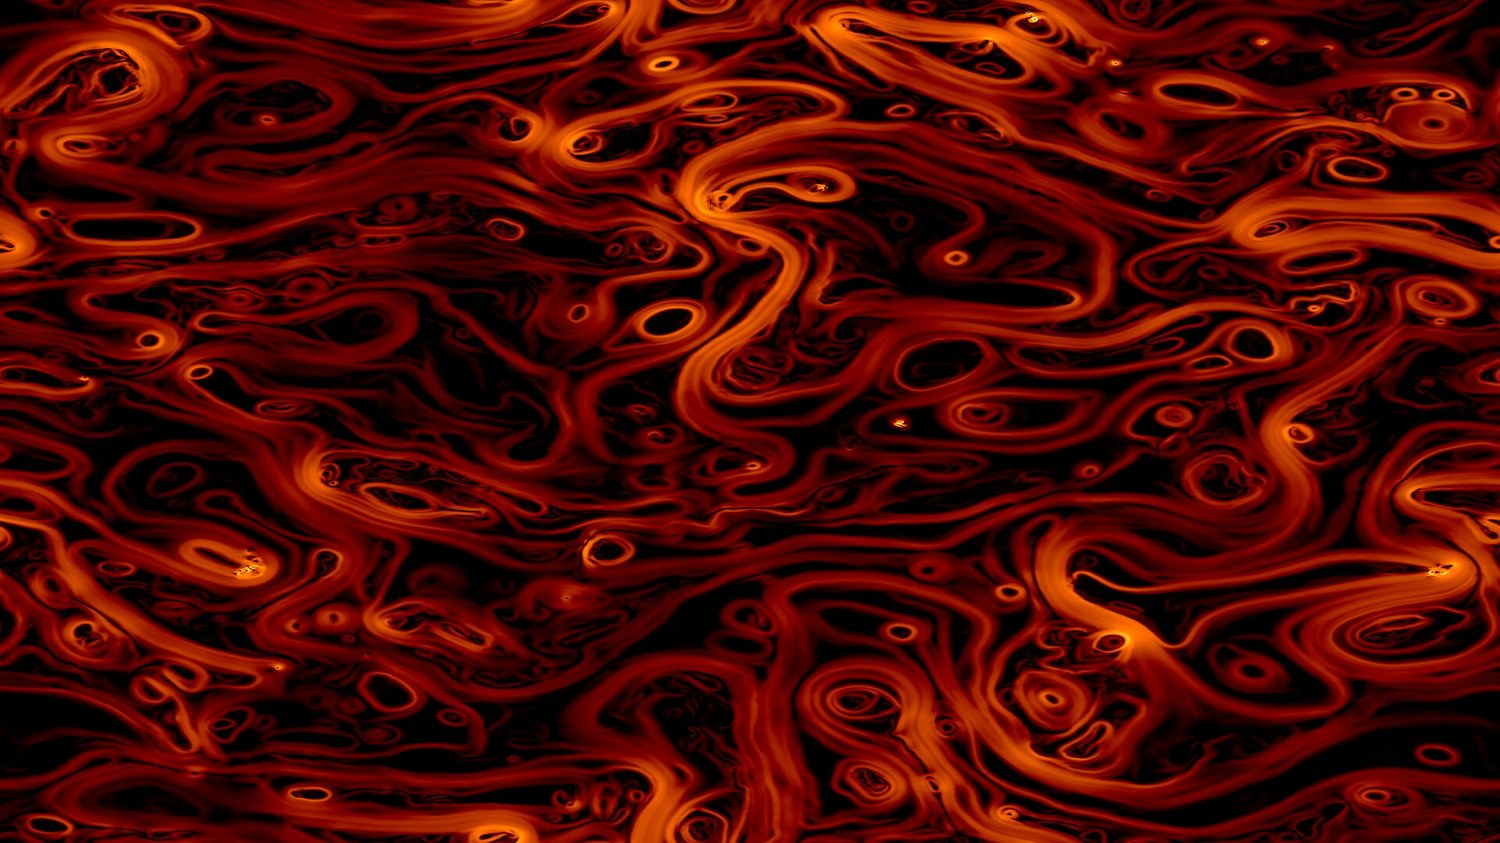
\includegraphics[width=0.72\textwidth]{../figures/magnetic_turbulence.jpg}
\caption{磁湍流：输运由哪一段波数贡献。把磁场的湍流结构画出来，才能理解「输运不是均匀发生」：能量从驱动尺度级联到耗散尺度，而真正贡献输运的往往只是其中一段波数——本节讨论的谱与级联，就是在这样的结构上做积分。}
\label{fig:photo-appaf}
\figsource{Giannandrea Inchingolo，CC BY-SA 4.0（Wikimedia Commons）}
\end{figure}

\section{混合长与饱和：上界与真值}
\label{sec:app-af-saturation}

湍流的线性增长率只给出时间尺度，要把增长率变成扩散系数，还需要一个长度。
最朴素的取法是「混合长」：涡有多大，粒子就一步走多远，于是
\begin{equation}
\gamma_{\max}=k_\theta\rho_s\frac{c_s}{L_n}=178057\ \mathrm{s^{-1}},
\qquad
\tau_c=\frac{1}{\gamma_{\max}}=5.61617\times10^{-6}\ \mathrm{s}=5.61617\ \mathrm{\mu s},
\label{eq:app-af-gamma}
\end{equation}
\begin{equation}
\chi_{\mathrm{mix}}=\frac{\gamma_{\max}}{k_\theta^2}=16.9004\ \mathrm{m^2\,s^{-1}},
\qquad
\frac{\chi_{\mathrm{mix}}}{\chi_{\mathrm{eff}}}=31.2658.
\label{eq:app-af-mixing}
\end{equation}
混合长比实验反推大 $31.2658$ 倍——这不是误差，而是\textbf{上界与真值的差别}。原因是饱和：
涡还没长到 $1/k_\theta$ 那么大，就被自己的非线性相互作用打碎了。

反过来用实验反推的扩散系数，可以问「有效的步长到底是多少」
\begin{equation}
\Delta r_{\mathrm{eff}}=\sqrt{\chi_{\mathrm{eff}}\tau_c}=1.74235\ \mathrm{mm},
\qquad
\frac{\Delta r_{\mathrm{eff}}}{\rho_s}=0.596134,
\qquad
\Delta r_{\mathrm{eff}}k_\theta=0.17884.
\label{eq:app-af-dreff}
\end{equation}
也就是说：混合长说「一步 $3.33333\,\rho_s$」，实测的有效步长只有 $0.596134\,\rho_s$，
差 $5.59$ 倍——\textbf{饱和把步长缩掉了一个因子，而不是把时间拉长}。

\begin{table}[htbp]
\centering
\small
\begin{tabular}{p{4.4cm}p{3.2cm}p{4.6cm}}
\toprule
量 & 值 & 说明 \\
\midrule
增长率 $\gamma_{\max}$ & $178057$ s$^{-1}$ & 取 $k_\theta\rho_sc_s/L_n$，与 $\omega_*$ 同阶 \\
相关时间 $\tau_c$ & $5.61617$ $\mu$s & $1/\gamma_{\max}$ \\
混合长步长 $1/k_\theta$ & $9.74246$ mm & $=3.33333\,\rho_s$ \\
混合长扩散 $\chi_{\mathrm{mix}}$ & $16.9004$ m$^2$s$^{-1}$ & 高估 $31.2658$ 倍 \\
有效步长 $\Delta r_{\mathrm{eff}}$ & $1.74235$ mm & 由 $\chi_{\mathrm{eff}}\tau_c$ 反推 \\
涨落水平（声明）$\delta n/n$ & $0.01$ & $(\delta n/n)^2$ 定标给 $0.00169004$ m$^2$s$^{-1}$ \\
\bottomrule
\end{tabular}
\caption{混合长量级链。注意最后一行：只把涨落水平乘进去会算出偏小的扩散系数，
说明「涨落水平」与「步长」不是两个独立的旋钮——它们是同一个饱和过程的两个侧面。}
\label{tab:app-af-saturation}
\end{table}

\begin{tip}{混合长是上界，不是预言}{tip-app-af-mixing}
$\chi_{\mathrm{mix}}/\chi_{\mathrm{eff}}=31.2658$ 这个数不要背成「混合长错了 30 倍」，
要记成「混合长给的是上限，真值由饱和机制决定」。判断一个湍流定标能不能用，
就看去掉饱和因子之后它还能不能对上量级——本工作点能，所以回旋玻姆定标在工程上够用。
\end{tip}

{\footnotesize
\textbf{出处：}混合长与饱和的讨论参照 Horton \emph{Rev. Mod. Phys.} \textbf{71} (1999) 735 与
Connor \& Wilson \emph{Plasma Phys. Control. Fusion} \textbf{36} (1994) 719。
「上界与真值」的口径与附录 AC 的截断误差、附录 AD 的气球模上限同一思路。
}

\section{带状流与剪切抑制}
\label{sec:app-af-zonal}

湍流并不是「越乱越输运」。它自己会长出\textbf{带状流}：环向对称、径向有限宽度的
$E\times B$ 流，把湍流涡沿径向撕开。先算这个流的速度，取附录 AD 的径向电场口径
$E_r=53.2405$ kV/m
\begin{equation}
v_{\mathrm{zf}}=\frac{E_r}{B}=\frac{53240.5}{5.3}=10045.4\ \mathrm{m\,s^{-1}},
\label{eq:app-af-vzf}
\end{equation}
剪切率取决于这个速度在多大径向尺度上变化
\begin{equation}
\gamma_E=\frac{v_{\mathrm{zf}}}{\Delta r},
\qquad
\gamma_E(\Delta r=\rho_i)=2.43031\times10^{6}\ \mathrm{s^{-1}},
\qquad
\frac{\gamma_E}{\gamma_{\max}}=13.649,
\label{eq:app-af-gammae}
\end{equation}
判据是 $\gamma_E\gtrsim\gamma_{\max}$：剪切率超过增长率，涡还没长大就被拉断。本工作点用
$\rho_i$ 作尺度时满足（$13.649$ 倍），但若把尺度放大到 $a/10=0.2$ m，
剪切率掉到 $50226.9$ s$^{-1}$，只有增长率的 $0.282083$ 倍——\textbf{抑制失效}。两种取法的分界尺度是
\begin{equation}
\Delta r_*=\frac{v_{\mathrm{zf}}}{\gamma_{\max}}=56.4165\ \mathrm{mm}=13.649\,\rho_i .
\label{eq:app-af-suppress}
\end{equation}
也就是说，带状流必须「细」才有效：径向宽度一旦超过十几个离子回旋半径，它自己就变成了
一个慢变的剪切层，对湍流不再有抑制作用。

\begin{table}[htbp]
\centering
\small
\begin{tabular}{p{3.4cm}p{3.4cm}p{3.0cm}p{3.4cm}}
\toprule
径向尺度 $\Delta r$ & $\gamma_E$ & $\gamma_E/\gamma_{\max}$ & 是否抑制 \\
\midrule
$\rho_i=4.13338$ mm & $2.43031\times10^{6}$ s$^{-1}$ & $13.649$ & 是 \\
$a/10=0.2$ m & $50226.9$ s$^{-1}$ & $0.282083$ & 否 \\
分界 $\Delta r_*=56.4165$ mm & $178057$ s$^{-1}$ & $1$ & 临界 \\
\bottomrule
\end{tabular}
\caption{剪切抑制判据。注意分界尺度 $56.4165$ mm 是 $13.649\,\rho_i$，
它同时是「$\gamma_E=\gamma_{\max}$」和「$\Delta r_*/\rho_i=\gamma_E/\gamma_{\max}$」两种写法的交点。}
\label{tab:app-af-zonal}
\end{table}

\begin{tip}{带状流是湍流自己长出来的「刹车」}{tip-app-af-zonal}
带状流不需要外部驱动：它是湍流通过雷诺胁强把能量从涡尺度转移到环向对称分量上的结果。
这构成一个负反馈回路——湍流越强，带状流越强，剪切越大，湍流被压回去。
所以把输运写成「$\chi\propto$ 梯度」的单调函数一定是错的：\textbf{它自己带刹车}。
\end{tip}

{\footnotesize
\textbf{出处：}带状流与 $E\times B$ 剪切抑制判据参照 Biglari、Diamond \& Terry
\emph{Phys. Fluids B} \textbf{2} (1990) 1、Hahm \& Burrell \emph{Phys. Plasmas} \textbf{2} (1995) 1648
与 Burrell \emph{Phys. Plasmas} \textbf{4} (1997) 1499。
径向电场口径与附录 AD 一致。
}

\begin{figure}[htbp]
\centering
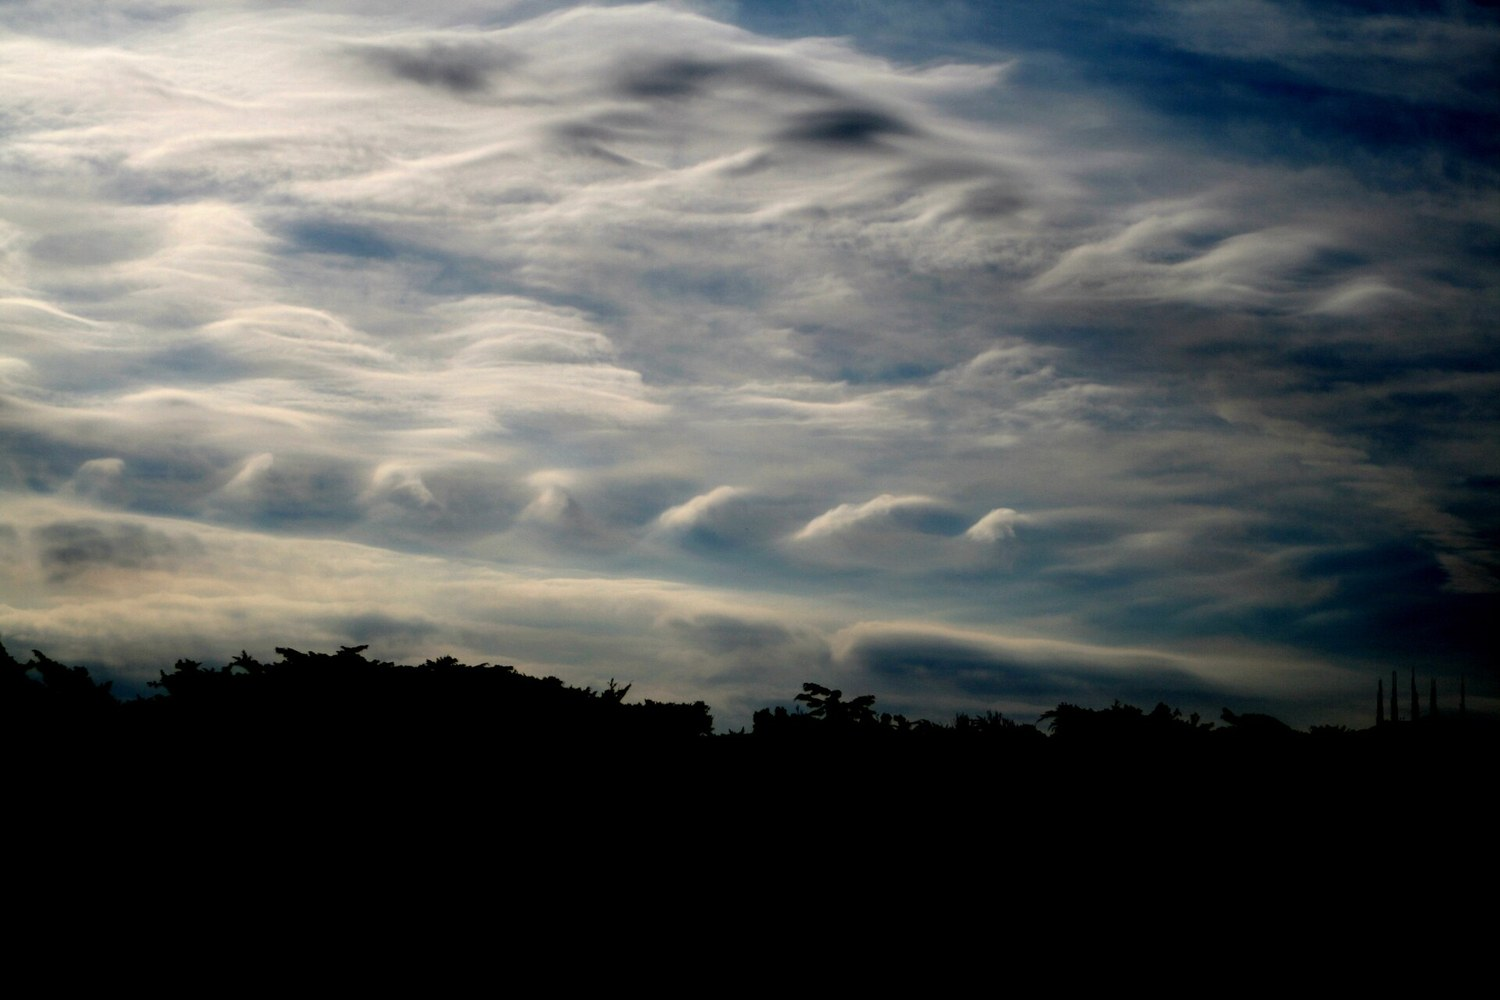
\includegraphics[width=0.72\textwidth]{../figures/af_kelvin_helmholtz.jpg}
\caption{湍流不是无序：能量先在大尺度生成，再逐级传到小尺度耗散掉。大气里这排卷起的云街，就是同一套级联在眼前发生——本节要问的是，输运由哪一段波数买单。}
\label{fig:photo-appaf3}
\figsource{Brocken Inaglory，CC BY-SA 3.0（Wikimedia Commons）}
\end{figure}

\section{谱与级联：输运由哪一段波数贡献}
\label{sec:app-af-spectrum}

把湍流写成波数谱 $S(k)$，输运的热流权重是 $k^2S(k)$（多一个 $k^2$ 来自 $\nabla$ 与体积因子）。
漂移波湍流的谱指数不是任意的：二维情形下熵级串给
\begin{equation}
S(k)\propto k^{-3},
\qquad\Longrightarrow\qquad
k^2S(k)\propto k^{-1},
\label{eq:app-af-spectrum}
\end{equation}
而逆能量级串与三维 Kolmogorov 级串给 $S(k)\propto k^{-5/3}$（文献值，声明）。
这两种谱的差别直接决定「输运由哪一段波数贡献」：
\begin{equation}
\frac{\int_{0.1}^{0.5}k^2S(k)\,\mathrm{d}k}{\int_{0.1}^{1.0}k^2S(k)\,\mathrm{d}k}
=\frac{\ln(0.5/0.1)}{\ln(1.0/0.1)}=\frac{\ln 5}{\ln 10}=0.69897,
\label{eq:app-af-flux}
\end{equation}
按 $k^{-1}$ 权重，$k_\theta\rho_s\le0.5$ 这一段就吃掉了 $69.897\%$ 的输运，
剩下的 $30.103\%$ 由 $0.5$--$1.0$ 段贡献。注意这个积分用的是 $k^{-1}$，
换成一个更平的谱（$S\propto k^{-5/3}$，权重 $k^{1/3}$）时高波数那一段的份额会明显上升——
\textbf{所以「哪一段贡献最大」这个问题的答案，取决于你把谱指数取成多少}。
这也是为什么回旋动理学的长波展开（附录 AE）只在工程精度下站得住：它默认了权重的重心在长波。

\begin{table}[htbp]
\centering
\small
\begin{tabular}{p{3.6cm}p{3.0cm}p{3.4cm}p{3.2cm}}
\toprule
谱 & $S(k)$ 指数 & $k^2S(k)$ 权重 & 含义 \\
\midrule
二维熵级串 & $-3$ & $\propto k^{-1}$ & 长波占 $69.897\%$（$k\le0.5$），余 $30.103\%$ \\
逆能量级串 & $-5/3$ & $\propto k^{1/3}$ & 高波数份额上升（长波不再独占） \\
三维 Kolmogorov & $-5/3$ & $\propto k^{1/3}$ & 各向同性惯性区 \\
\bottomrule
\end{tabular}
\caption{谱指数与输运权重。第一行的两个比例是 $k^{-1}$ 权重下
$0.1$--$0.5$ 与 $0.5$--$1.0$ 两段的份额；谱越平，输运越向高波数移动。}
\label{tab:app-af-spectrum}
\end{table}

\begin{tip}{谱指数不是装饰，它决定输运集中在哪里}{tip-app-af-spectrum}
同一句「湍流输运」在 $k^{-3}$ 与 $k^{-5/3}$ 两种谱下对应的物理完全一样，
但要把网格、诊断波数窗口、混合长截断点定在哪里，答案都在这一段。
做模拟前先问「我的谱指数是多少」，比先调系数有效。
\end{tip}

{\footnotesize
\textbf{出处：}二维漂移波熵级串与逆能量级串的谱指数参照 Kraichnan \emph{Phys. Fluids}
\textbf{10} (1967) 1417 与 Hasegawa \& Mima \emph{Phys. Fluids} \textbf{21} (1978) 87，三维 Kolmogorov 谱参照 Kolmogorov \emph{Dokl. Akad. Nauk SSSR} \textbf{30} (1941) 301。
}

\section{估算练习}
\label{sec:app-af-problems}

\textbf{练习 1} 把磁场从 $5.3$ T 提到 $10$ T，其他参数不变。先算 $\rho_s$ 与 $\chi_{\mathrm{gB}}$，
再判断「约束会变好多少」。

\textbf{练习 2} 把温度梯度长度从 $0.5$ m 压到 $0.3$ m（梯度更陡）。
算 $R/L_T$ 与超临界倍数，并说明芯部温度会不会跟着涨 $1.67$ 倍。

\textbf{练习 3} 用 $\chi_{\mathrm{eff}}$ 与线性增长率反推「有效步长」，并说明它与混合长的差别。

\textbf{练习 4} $B$ 翻倍时 $\chi_{\mathrm{gB}}$ 与 $\chi_B$ 各按什么幂次变化？二者之比变几倍？

\textbf{练习 5} 若要把有效扩散系数压到 $\chi_{\mathrm{eff}}=1$ m$^2$s$^{-1}$，
对应的能量约束时间是多少？与现在的 $3.7$ s 相比是变好还是变差？

\textbf{练习 6} 用 $E_r=53.2405$ kV/m 算带状流速度与剪切率，
并求「剪切率等于增长率」的临界径向尺度。

\textbf{解答 1} $B=10$ T 时 $\omega_{ci}=3.83153\times10^{8}$ rad s$^{-1}$、
$\rho_s=1.54905$ mm、$k_\theta=193.667$ m$^{-1}$；
$\chi_B=57.4625$ m$^2$s$^{-1}$、$\chi_{\mathrm{gB}}=0.712099$ m$^2$s$^{-1}$，
两者之比 $80.6945$。$\chi_{\mathrm{gB}}$ 随 $B$ 缩小 $3.55999$ 倍、$\chi_B$ 缩小 $1.88679$ 倍，
而 $\omega_*$ 不变（固定 $k_\theta\rho_s$ 时 $178057$ rad s$^{-1}$）。
所以「约束变好」的幅度取决于你用哪个定标：玻姆好得慢，回旋玻姆好得快。

\textbf{解答 2} $R/L_T=20.6667$，超临界 $3.13333$ 倍；$L_{T,\mathrm{crit}}=1.24$ m 不变，
实际梯度是临界值的 $4.13333$ 倍。温度不会涨 $1.67$ 倍——\textbf{临界梯度会把剖面钉住}，
多出来的加热主要变成输运而不是温度。

\textbf{解答 3} 有效步长 $\Delta r_{\mathrm{eff}}=\sqrt{\chi_{\mathrm{eff}}\tau_c}=1.74235$ mm，
即 $0.596134\,\rho_s$；而混合长给 $1/k_\theta=9.74246$ mm $=3.33333\,\rho_s$。
二者差 $5.59$ 倍：混合长给的是上限，饱和把步长缩小了。

\textbf{解答 4} $\chi_{\mathrm{gB}}=\rho_s^2c_s/a\propto B^{-2}$（因为 $\rho_s\propto B^{-1}$），
所以 $B$ 翻倍时 $\chi_{\mathrm{gB}}$ 变 $0.25$ 倍；$\chi_B\propto B^{-1}$，变 $0.5$ 倍；二者之比变 $2$ 倍。

\textbf{解答 5} $\tau_E=a^2/(2\chi_{\mathrm{eff}})=2$ s，是现在 $3.7$ s 的 $0.540541$ 倍——
\textbf{更短，约束更差}。要把约束变好，必须让 $\chi_{\mathrm{eff}}$ 比现在再小。

\textbf{解答 6} $v_{\mathrm{zf}}=E_r/B=10045.4$ m s$^{-1}$；
取 $\rho_i$ 为径向尺度时 $\gamma_E=2.43031\times10^{6}$ s$^{-1}=13.649\,\gamma_{\max}$（能抑制）；
临界尺度 $\Delta r_*=56.4165$ mm，比 $\rho_i=4.13338$ mm 大 $13.649$ 倍。

\section{来源、分级与版权说明}
\label{sec:app-af-source}

\begingroup\small
本附录的数值分三级，每一级的可核验程度不同：

\begin{table}[htbp]
\centering
\small
\begin{tabular}{p{2.6cm}p{4.2cm}p{2.6cm}p{4.4cm}}
\toprule
级别 & 内容 & 例子 & 可核验性 \\
\midrule
现算级 & 由 \texttt{tools/\allowbreak{}calc/\allowbreak{}appAF\_calc.py} 从工作点算出 & $\rho_s=2.92274$ mm、$\chi_{\mathrm{mix}}=16.9004$ m$^2$s$^{-1}$ & 可逐位复算 \\
声明级 & 脚本顶部的输入或文献量级 & $L_n=1.0$ m、$\eta_{i,\mathrm{crit}}=1.5$、谱指数 $-3/-5/3$ & 可改输入重算 \\
文献级 & 定标系数的适用范围 & 回旋玻姆系数、混合长饱和因子 & 需查原文 \\
\bottomrule
\end{tabular}
\caption{数值分级。第三级的量在本附录只作量级对照，不作为结论使用。}
\label{tab:app-af-source}
\end{table}

\textbf{分级说明}：本附录只讲「为什么约束就是这个数」的量级链，不给输运系数的第一性原理求解；
$\chi_{\mathrm{eff}}$ 是实验反推的等效扩散系数，不是从湍流方程算出来的。混合长、临界梯度、
谱指数都按声明值使用，改动它们会改动量级但不改动结论的方向。

\textbf{不复制}：本附录不复制任何原书的文字、编号、插图与数据表；
不复制任何实验装置的剖面图与谱图；不复制任何湍流模拟的原始数据；
不复制任何定标律的拟合表——只借鉴「结构、判据形式与量级关系」，文字与数值自拟并独立复算。

\begin{tip}{诚实地说清「本附录不给什么」}{tip-app-af-honest}
本附录不给：非线性湍流的解析解、输运系数的第一性原理计算、任何装置的具体剖面。
给的是：把「梯度有多陡、涡有多大、剪切有多强」串成一条能自己算的量级链，
以及每个环节的上界与真值差多少（本工作点：混合长高估 $31.2658$ 倍）。
\end{tip}

\textbf{出处：}回旋玻姆定标与 $\rho_s$ 口径参照 Wesson \emph{Tokamaks}（第 4 版，2011，第 12 章）
与 Helander \& Sigmar \emph{Collisional Transport in Magnetized Plasmas}（2002，第 1 章）。
临界梯度与刚性的综述参照 Dimits 等 \emph{Phys. Plasmas} \textbf{7} (2000) 969 与
Doyle 等 \emph{Nucl. Fusion} \textbf{47} (2007) S18。
$\rho_s$ 与 $\rho_i$ 的口径与附录 AE 一致。
\endgroup